\documentclass{../../zirkelblatt1415}
\setlength\parskip{\medskipamount}
\setlength\parindent{0pt}

\usepackage{geometry}
\geometry{top=1.5cm,bottom=1cm,left=2cm,right=2cm}
\pagestyle{empty}

\usepackage{tikz}
\usetikzlibrary{calc}

\begin{document}
\sffamily

\newcommand{\zettel}[1]{
  {\Huge \textbf{Cosmic Call (\thepage/23)}\par}
  \bigskip

  \includegraphics[width=\textwidth]{images/p#1}

  \begin{tikzpicture}[remember picture, overlay]
    \node [anchor=south west, outer sep=0pt, inner sep=0pt]  at ($(current page.south west) +(0.2cm,0.3cm)$)
        {
\includegraphics[height=2cm]{gregor-gespiegelt-klein}};
  \end{tikzpicture}

  \newpage
}

\newcommand{\zettelD}[1]{
  {\Huge \textbf{Cosmic Call (\thepage/23)}\par}
  \bigskip

  \includegraphics[width=\textwidth]{images/p#1}
  \bigskip

  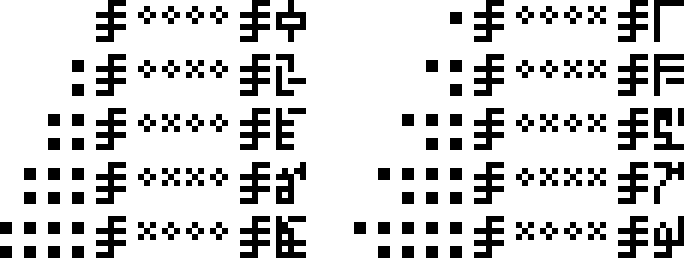
\includegraphics[width=\textwidth]{images/digits}

  \begin{tikzpicture}[remember picture, overlay]
    \node [anchor=south west, outer sep=0pt, inner sep=0pt]  at ($(current page.south west) +(0.2cm,0.3cm)$)
        {
\includegraphics[height=2cm]{gregor-gespiegelt-klein}};
  \end{tikzpicture}

  \newpage
}

\centering
\zettel{01}
\zettelD{02}
\zettelD{03}
\zettelD{04}
\zettelD{05}
\zettelD{06}
\zettelD{07}
\zettelD{08}
\zettelD{09}
\zettelD{10}
\zettelD{11}
\zettelD{12}
\zettelD{13}
\zettelD{14}
\zettelD{15}
\zettelD{16}
\zettelD{17}
\zettelD{18}
\zettelD{19}
\zettelD{20}
\zettelD{21}
\zettelD{22}
\zettelD{23}

\end{document}
